\documentclass[12pt]{exam}

% essential packages
\usepackage{fullpage} % margin formatting
\usepackage{enumitem} % configure enumerate and itemize
\usepackage{amsmath, amsfonts, amssymb, mathtools} % math symbols
\usepackage{xcolor, colortbl} % colors, including in tables
\usepackage{makecell} % thicker \Xhline in table
\usepackage{graphicx} % images, resizing

% sometimes needed packages
\usepackage{hyperref} % hyperlinks
% \hypersetup{colorlinks=true, urlcolor=blue}
% \usepackage{logicproof} % natural deduction
\usepackage{tikz} % drawing graphs
\usetikzlibrary{positioning}
% \usepackage{multicol}
% \usepackage{algpseudocode} % pseudocode

% paragraph formatting
\setlength{\parskip}{6pt}
\setlength{\parindent}{0cm}

% newline after Solution:
\renewcommand{\solutiontitle}{\noindent\textbf{Solution:}\par\noindent}

% less space before itemize/enumerate
\setlist{topsep=0pt}

% creates \filcl to grey out cells for groupwork grading
\newcommand{\filcl}{\cellcolor{gray!25}}

% creates \probnum to get the problem number
\newcounter{probnumcount}
\setcounter{probnumcount}{1}
\newcommand{\probnum}{\arabic{probnumcount}. \addtocounter{probnumcount}{1}}

% use roman numerals by default
\setlist[enumerate]{label={(\roman*)}}

% creates custom list environments for grading guidelines, question parts
\newlist{guidelines}{itemize}{1}
\setlist[guidelines]{label={}, left=0pt .. \parindent, nosep}
\newlist{gwguidelines}{enumerate}{1}
\setlist[gwguidelines]{label={(\roman*)}, nosep}
\newlist{qparts}{enumerate}{2}
\setlist[qparts]{label={(\alph*)}}
\newlist{qsubparts}{enumerate}{2}
\setlist[qsubparts]{label={(\roman*)}}
\newlist{stmts}{enumerate}{1}
\setlist[stmts]{label={(\roman*)}, nosep}
\newlist{pflist}{itemize}{4}
\setlist[pflist]{label={$\bullet$}, nosep}
\newlist{enumpflist}{enumerate}{4}
\setlist[enumpflist]{label={(\arabic*)}, nosep}

\printanswers

\begin{document}
%%%%%%%%%%%%%%% TITLE PAGE %%%%%%%%%%%%%%%
\title{EECS 203: Discrete Mathematics\\
  Fall 2023\\
  Homework 5}
\date{}
\author{}
\maketitle
\vspace{-50pt}
\begin{center}
  \huge Due \textbf{Thursday, October. 12}, 10:00 pm\\
\Large No late homework accepted past midnight.\\
\vspace{10pt}
\large Number of Problems: $7+2$
\hspace{3cm}
Total Points: $100+20$
\end{center}
\vspace{25pt}
\begin{itemize}
    \item \textbf{Match your pages!} Your submission time is when you upload the file, so the time you take to match pages doesn't count against you.
    \item Submit this assignment (and any regrade requests later) on Gradescope. 
    \item Justify your answers and show your work (unless a question says otherwise).
    \item By submitting this homework, you agree that you are in compliance with the Engineering Honor Code and the Course Policies for 203, and that you are submitting your own work.
    \item Check the syllabus for full details.
\end{itemize}
\newpage
%%%%%%%%%%%%%%% TITLE PAGE %%%%%%%%%%%%%%% 

\section*{Individual Portion}

\subsection*{\probnum Induction Construction [16 points]} 
Let $P(n)$ be the statement that $1 \cdot 1! + 2 \cdot 2!+\dots+ n \cdot n! = (n + 1)! - 1$
whenever $n$ is a positive integer. In this problem, we will prove this statement via weak induction.
\begin{qparts}
    \item What is the statement $P(1)$?
    \item Show that $P(1)$ is true, which is the base case for our inductive step.
    \item In the base case we prove $P(1)$; what do you need to prove in the inductive step?
    \item What is the inductive hypothesis for your proof?
    \item Complete the inductive step, indicating where you used the inductive hypothesis.
    \item Explain why this proof shows $P(n)$ is true for all positive integers $n$.
\end{qparts}

\begin{solution}
    \begin{qparts}
        \item $P(1)$: $1 \cdot 1! = (1+1)!  - 1$.
        \item For $P(1)$, LHS =  1\\
                    RHS = $2! - 1 = 2 \cdot 1 - 1 = 1$.\\.
                    $\therefore$ LHS = RHS.
                    $\therefore$ $P(1)$ is true.
        \item We need to prove that $P(k) \rightarrow P(k+1)$ for any integer $n$ which is $\geq$ 1.
        \item The inductive hypothesis: Assume $P(k)$: $1 \cdot 1! + 2 \cdot 2!+\dots+ n \cdot n! = (n + 1)! - 1$.
        \item Let $k$ be an arbitrary positive integer.\\
            Assume $P(k)$: $1 \cdot 1! + 2 \cdot 2!+\dots+ n \cdot n! = (n + 1)! - 1$\\
            Want to show: $P(k+1)$: $1 \cdot 1! + 2 \cdot 2!+\dots+ n \cdot n! + (n+1) \cdot (n+1)! = (n + 1 + 1)! - 1$\\
            Using $P(n)$ we know: 
            \begin{align*}
                1 \cdot 1! + 2 \cdot 2!+\dots+ n \cdot n! + (n+1) \cdot (n+1)! &= (n + 1)! - 1 + (n+1) \cdot (n + 1)! \\
                &= (n+1)! (1 + n + 1) + 1\\
                &= (n + 1 + 1)\cdot (n+1) \cdot n \cdot (n-1) \cdot \cdots \cdot 1 -1\\
                &= (n + 1 + 1)! -1
            \end{align*}
            Thus $P(k) \rightarrow P(k+1)$ for any integer $n$ which is $\geq$ 1.
        \item It is because that: (1) $P(1)$: $1 \cdot 1! = (1+1)!  - 1$.\\
            (2)$P(k) \rightarrow P(k+1)$ for any integer $n$ which is $\geq$ 1.\\
            Therefore $P(1) \rightarrow P(2) \rightarrow P(3) \cdots \rightarrow P(n)$\\
            Where $n$ can be any positive integer.\\
            $\therefore$ Since we know (1) is true and (2) is true, $P(n)$ is true for all positive integers $n$.

    \end{qparts}
\end{solution}


\subsection*{\probnum Base Two Blues [14 points]}
Prove using mathematical induction that $\text{log}_2 (n) < n$ for every positive integer $n$. You may assume that the base-2 logarithm function is strictly increasing on its domain.

\textbf{Fun Fact:} $\text{log}_b(n) < n$ is actually true for every positive real number $n$ and arbitrary base $b>1$, but we're asking you to prove this by induction for the special case where $b =2$ and $n$ is a positive integer.

\begin{solution}
    Let $k$ be an arbitrary positive integer.\\
    Assume $P(k)$: $\log_2{k} < k$\\
    Want to show: $P(k+1):$ $\log_2{k+1} < k + 1$\\\\
    \textbf{Base Case:}\\
    $P(0): \log_2{1} < 1$ \\
    Since $\log_2{1} = 0 < 1$, base case is true.\\\\
    \textbf{Inductive Step:}\\
    Using the property of logarithm we know:
    \begin{align*}
        \log_2{(k+1)} &= \log_2{(\frac{k+1}{k} \cdot k)}\\
                    &= \log_2{\frac{k+1}{k}} + \log_2{ k}\\
                    &= \log_2{(1 + \frac{1}{k})} + \log_2{ k}
    \end{align*}
    Since $k$ is a positive integer, $k \geq 1$, $\frac{1}{k} \leq 1$, $\frac{1}{k} + 1\leq 2$\\
    $\therefore \log_2{(\frac{1}{k} + 1)} \leq 1$. \\
    Using $P(n)$ we know: $\log_2{k} < k$. \\
    And Since $\log_2{(\frac{1}{k} + 1)} \leq 1$ and $\log_2{k} < k$\\
    $log_2{(k+1)} = \log_2{(1 + \frac{1}{k})} + \log_2{ k} < k + 1$.\\
    Then we have proved that $P(K) \rightarrow P(k+1)$ for all positive integer $k$.\\\\
    Conclusion: $\text{log}_2 (n) < n$ for every positive integer $n$.
\end{solution}


\subsection*{\probnum Inductive Hypothe-six [15 points]}
Prove by weak induction that 6 divides $n^3 - n$ where $n$ is a nonnegative integer. Don't include unneeded base cases.

\begin{solution} 
    Let $k$ be an arbitrary nonnegative integer.\\
    Assume $P(k)$: $6 | (k^3 - k)$\\
    Want to show: $P(k+1)$: $6 | [(k+1)^3 - (k+1)]$\\\\
    \textbf{Base Case:}\\
    $P(0)$: $6 | 0^3 - 0$\\
    Since $0^3 - 0 = 0$, $6 | 0$, base case is true.\\\\
    \textbf{Inductive Step:}\\
    Since $P(k)$: $6 | (k^3 - k)$, for some integer $m$, $6m = (k^3 - k)$\\
    Then 
    \begin{align*}
        (k+1)^3 - (k+1) &= k^3 + 3k^2 + 3k + 1 - k - 1 \\
                        &= k^3 + 3k^2 + 2k \\
                        &= (k^3 - k) + 3k^2 + 3k \\
                        &= 6m + 3(k^2 + k)
                        &= 6m + 3k\cdot(k+1)
    \end{align*}
    Since $k$ is an integer, and integers consist of alternating odd numbers and even numbers, 
    one of $k$ and $k+1$ must be even. WLOG assume $k$ is even, then for some integer $p$, $k=2p$. \\
    Then $(k+1)^3 - (k+1) = 6m + 3 \cdot 2p\cdot(k+1) = 6m + 6p\cdot (k + 1) = 6[m + p(k+1)]$\\
    Since $p,m,k$ are integers, $p(k+1)$ is an integer, $[m + p(k+1)]$ is an integer.\\
    Then $6 | [m + p(k+1)]$, i.e. $6 | [(k+1)^3 - (k+1)]$. \\
    Therefore we have proved that $P(k) \rightarrow P(k+1)$ for any nonnegative integer $k$.\\\\
    Conclusion: 6 divides $n^3 - n$ where $n$ is a nonnegative integer.
\end{solution}


\subsection*{\probnum Incorrect Strong Induction [14 points]}
For each of the following \textbf{incorrect} strong induction proofs, note where the strong induction proof breaks down and is incorrect.

\textbf{Hint:} Consider where the inductive step breaks down.

\begin{qparts}
    \item Proving for every nonnegative integer $n$, $P(n)\colon 3n = 0$.
    
    \textbf{Inductive Step:}
    
    Assume that $P(j)\colon 3j = 0$ for all nonnegative integers $j$ with $0 \leq j \leq k$. We wish to show $P(k+1)$. We will rewrite $k+1 = a + b$ where $a$ and $b$ are nonnegative integers less than $k+1$. Thus, $3 \cdot (k+1) = 3 \cdot (a+b) = 3a + 3b = 0 + 0 = 0$, therefore $P(k+1)$ is proven.
    
    \textbf{Base Case:} $P(0)\colon 3 \cdot 0 = 0$
    
    Since we have shown the basis step and the inductive step, we have proved for every nonnegative integer $n$, $P(n): 3n = 0$.
    
    \item Proving that every cent value above 3 cents can be formed using just 3-cent and 4-cent stamps.
    
    \textbf{Inductive Step:}
    
    Assume we can form cent values of $j$ cents for all $3 \leq j \leq k$ using just 3-cent and 4-cent stamps. We wish to show we can form $k+1$ cents using just 3-cent and 4-cent stamps. We can form a $k+1$ cent value by replacing 1 3-cent stamp with 1 4-cent stamp or by replacing 2 4-cent stamps with 3 3-cent stamps.
    
    \textbf{Base Case:}
    
    We can form cent values of 3-cents using one 3-cent stamp and we can form cent values of 4-cents using one 4-cent stamp. This covers our two base cases.
    
    Since we have shown the basis step and the inductive step, we have proved every cent value above 3 cents can be formed using just 3-cent and 4-cent stamps.
\end{qparts}

\begin{solution}
    \begin{qparts}
        \item 
            The proof breaks down from the base case when we induce $P(0) \rightarrow P(1)$.\\
            At this point, $k + 1 = 1$, but we cannot find 
            two integers $a$ and $b$ that are less than 1 while they add up to 1.If $a$, $b$ are less than 1 and nonnegative, 
            then they can only be both 0. Then they add to to 0 but not 1.\\
            Therefore the proof is incorrect.

        \item 
            The proof breaks down when we induce $(P(3) \land P(4)) \rightarrow P(5)$.\\
            The inductive step states that we can form a $k + 1$ cent value by 
            replacing 1 3-cent stamp with 1 4-cent or by replacing 2 4-cent stamps with 3 3-cent stam. 
            But at this point, we only have one 4-cent and can not apply the induction.\\
            Therefore the proof is incorrect.
            
    \end{qparts}
\end{solution}


\subsection*{\probnum Chopping Ice [15 points]}
Claire doesn't have an ice tray, so she makes ice by freezing water into a rectangle and then dividing the rectangle into grid-aligned cells. She would like to divide her block of ice into $n$ rows and $m$ columns quickly, before the ice melts! See the image below for an example.
\begin{center}
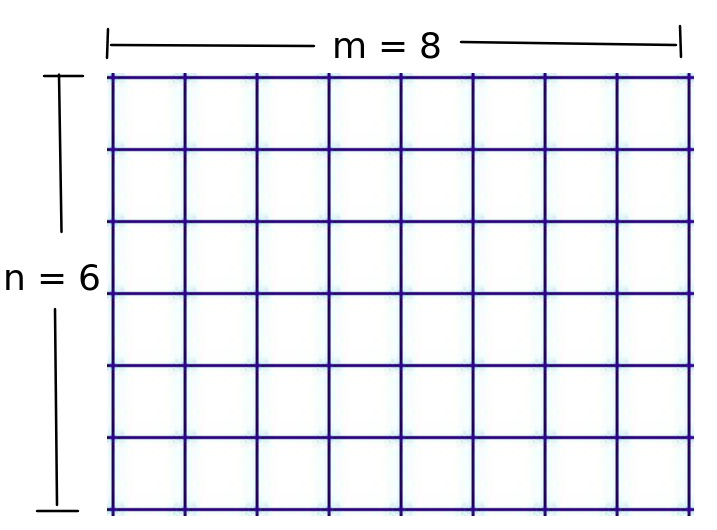
\includegraphics[scale = 0.3]{ice.png}
\end{center}
\begin{qparts}
    \item State the number of cuts Claire needs to make to divide her ice block into $n \times m$ cells. One cut means splitting a single rectangle into two rectangles. In other words, you may NOT make a single cut across multiple pieces of ice. You may use $n$ and/or $m$ in your answer.
    
    \item Prove your answer from part (a).
\end{qparts}

\begin{solution} 
    \begin{qparts}
        \item $(m-1) \cdot (n-1) = mn -m -n + 1$\\
             $m,n$ are positive integers.
        \item 
    \end{qparts}

\end{solution}


\subsection*{\probnum Pastry Recurrence [12 points]}
A baker decorates a cookie in 2 minutes, a cupcake in 3 minutes, and a pie in 3 minutes.
Let $a_n$ denote the number of distinct ways the baker decorates pastries in exactly $n$ minutes for $n \geq 0$ (where order matters).
\begin{qparts}
    \item Find a recurrence relation for $a_n$.
    \item What are the initial conditions? Use the fewest initial conditions necessary. 
\end{qparts}

\begin{solution}

\end{solution}


\subsection*{\probnum Raven's Wrestlers [14 points]}
Raven has $n$ weeks to build her wrestling figure collection.  Every week, Raven buys one item to add to her collection.  There are 4 different types of things she can buy: Figures, T-shirts for her wrestlers to wear, Weapons for them to fight with, or Display Stands to show them off on her shelves.
\begin{itemize}
    \item Her shelves can fit 2 Stands nicely, so when she buys a Display Stand, she will always buy a second one the next week to finish the shelf.  Additionally, the week after buying the second Stand, she will buy something other than a Display Stand (they aren't as exciting to buy)
    \item When she buys a Figure, she gets very excited about it and wants to buy a new T-shirt for it to wear the following week.
\end{itemize}
Let $a_n$ represent the number of ways Raven can buy items across the $n$ weeks (where $n\geq 0$)
\begin{qparts}
    \item Find a recurrence relation for $a_n$.
    \item Which terms would need to be defined with initial conditions (no need to find the value, just which terms)
\end{qparts}
\textit{Note 1:} Buying the same items in a different order counts as a different way of buying items.  We treat all items in a category as identical.

\textit{Note 2:} on week $n$, Raven will not buy a Figure (because she knows she will miss buying a T-shirt) or a Stand (what a sad way to end the collection).  This information is not needed for the simplest solutions, but some alternate solutions may need to know this.

\begin{solution}

\end{solution}


\pagebreak

\setcounter{probnumcount}{1}
\section*{Groupwork}
\subsection*{\probnum Grade Groupwork 4}
Using the solutions and Grading Guidelines, grade your Groupwork 4:
\begin{itemize}
    \item Mark up your past groupwork and submit it with this one.
    \item Write whether your submission achieved each rubric item. If it didn't achieve one, say why not.
    \item Use the table below to calculate scores.
    \item For extra credit, write positive comment(s) about your work.
    \item You don't have to redo problems correctly, but it is recommended!
    \item What if my group changed? \begin{itemize}
        \item If your current group submitted the same groupwork last time, grade it together.
        \item  If not, grade your version, which means submitting this groupwork assignment separately. You may discuss grading together.
    \end{itemize}
\end{itemize}

\begin{center}
\resizebox{\textwidth}{!}{\begin{tabular}{| c | c | c | c | c | c | c | c | c | c | c | c | c |}
\hline
 & (i) & (ii) & (iii) & (iv) & (v) & (vi) & (vii) & (viii) & (ix) & (x) & (xi) & Total:\\
\hline
Problem 2 & & & & & &\filcl &\filcl &\filcl &\filcl & \filcl& \filcl& \hspace{1cm}/20\\
\hline 
Problem 3 & & & & & & & &\filcl &\filcl & \filcl& \filcl& \hspace{1cm}/30\\
\Xhline{1.25pt}
Total: &\filcl &\filcl &\filcl &\filcl &\filcl &\filcl &\filcl &\filcl & \filcl& \filcl& \filcl&\hspace{1cm}/50\\
\hline
\end{tabular}}
\end{center}


\subsection*{\probnum Polly Gone [12 points]}

A convex polygon is a 2D shape with all straight edges such that any line segment between any two non-adjacent vertices passes entirely through its interior (see example picture below). Show via induction that the sum of the interior angles of a convex polygon with $n$ sides is $(n - 2) \cdot 180^{\circ}$. Don't include unneeded base cases.

\begin{center}
    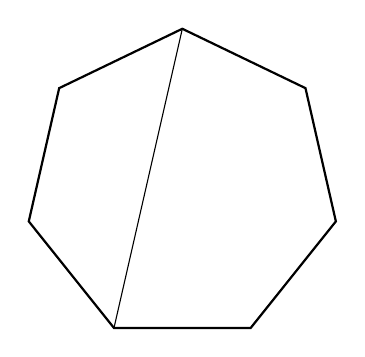
\begin{tikzpicture}[scale = 2]
        \draw[thick, black]  (0,1) -- (0.782,0.623) -- (0.975,-0.223)--(0.434,-0.9)--(-0.434,-0.9)--(-0.975,-0.223)--(-0.782,0.623)--cycle;
        \draw[thin,black] (0,1) -- (-0.434,-0.9);
    \end{tikzpicture}
\end{center}

\textbf{Hint 1}: It is helpful to know that a triangle's interior angles always sum to $180^{\circ}$. You may assume this is true for the problem.

\textbf{Hint 2}: In order to apply your inductive hypothesis to a convex polygon, you'll need to think of it in terms of smaller convex polygons. How can you make smaller polygons out of a big one?

\begin{solution}

\end{solution}


\smallskip
\subsection*{\probnum Running Recurrence [8 points]}
An EECS 203 student goes to lecture everyday. On each day, she always chooses exactly one method of transportation, and always chooses to walk, bike, or take a bus. She also follows additional rules:
\begin{itemize}
    \item She never walks two days in a row.
    \item If she takes the bus, she must have biked two days ago and walked a day ago.
\end{itemize}

Let $a_n$ denote the number of ways she can go to EECS 203 lecture across $n$ days for $n \geq 0$.
\begin{qparts}
    \item Find a recurrence relation for $a_n$.
    \item What are the initial conditions? Use the fewest initial conditions necessary.
\end{qparts}

\begin{solution}


\end{solution}

\end{document}
